\documentclass[letterpaper,12pt,fleqn]{article}
\usepackage{matharticle}
\usepackage{tikz}
\pagestyle{plain}
\newcommand{\T}{\mathscr{T}}
\renewcommand{\S}{\mathcal{S}}
\newcommand{\B}{\mathcal{B}}
\newcommand{\e}{\epsilon}
\renewcommand{\a}{\alpha}
\newcommand{\A}{A}
\renewcommand{\l}{\lambda}
\renewcommand{\L}{\Lambda}
\begin{document}
Cavallaro, Jeffery \\
Math 275A \\
Homework \#4

\bigskip

\begin{theorem}[3.1]
  Let \((X,\T)\) be a topological space and let \(\B\subset\T\).  \(\B\) is a basis for \(\T\) iff:
  \[\forall\,U\in\T,\forall\,p\in U,\exists\,V\in\B,p\in V\subset U\]
\end{theorem}

\begin{proof}
  \begin{description}
  \item[]
  \item[\(\implies\)] Assume that \(\B\) is a basis for \(\T\).

    Assume \(U\in\T\).  This means that there exists \(\B_U\subset\B\) such that \(U=\bigcup\B_U\).  Now, assume
    that \(p\in U\).  Thus, \(p\in\bigcup\B_U\) and therefore there exists some \(V\in\B_U\) such that
    \(p\in V\subset U\).

  \item[\(\impliedby\)] Assume \(\forall\,U\in\T,\forall\,p\in U,\exists\,V\in\B,p\in V\subset U\)

    Assume that \(U\in\T\).  For each \(p\in U\), choose a set \(V_p\in\B\) such that \(p\in V_p\subset U\).  Thus
    \(U=\bigcup_{p\in U}V_p\) and so every \(U\in\T\) is generated by \(\B\).  Therefore \(\B\) is a basis for
    \(\T\).
  \end{description}
\end{proof}

\begin{example}[Exercise 3.2]
  Let \(\T\) be the standard topology on \(\R\).  Show that the following are bases for \(\T\):
  \begin{enumerate}
  \item \(\B_1=\setb{(a,b)\subset\R}{a,b\in\Q}\)

    All the \((a,b)\) are open and hence \(\B_1\subset\T\).  So assume \(U\in\T\) and assume \(p\in U\).  Since
    \(U\) is open, there exists an open ball \(B(p,\e)\subset U\).  Since there exists an infinite number of
    rationals between any two reals, select two rationals \(a\in(p-\e,p)\) and \(b\in(p,p+\e)\).  Thus
    \((a,b)\in\B_1\) and \(p\in(a,b)\subset U\).  Therefore, by the previous theorem, \(\B_1\) is a basis for
    \(\T\).

  \item \(\B_2=\setb{(a,b)\cup(c,d)\subset\R}{a,b,c,d\in\R-\Q\ \text{and}\ a<b<c<d}\)

    All the \((a,b)\cup(c,d)\) are unions of open sets, so they are open as well and hence \(\B_2\subset\T\).  So
    assume \(U\in\T\) and assume \(p\in U\).  Since \(U\) is open, there exists an open ball \(B(p,\e)\in U\).
    Since there exists an infinite number of irrationals between any two real numbers, select four irrationals as
    follows:
    \begin{gather*}
      a\in(p-\e,p) \\
      b\in(p,p+\e) \\
      c\in(b,p+\e) \\
      d\in(c,p+\e)
    \end{gather*}
    Thus \(a<b<c<d\) and so \((a,b)\cup(c,d)\in\B_2\). Furthermore, \(p\in(a,b)\cup(c,d)\subset U\).  Therefore, by
    the previous theorem, \(\B_2\) is a basis for \(\T\).
  \end{enumerate}
\end{example}

\begin{theorem}[3.3]    
  Let \(X\) be a set and let \(\B\subset2^X\).  \(\B\) is a basis for some topology \(\T\) on \(X\) iff:
  \begin{enumerate}
  \item \(\forall\,p\in X,\exists\,V_p\in\B,p\in V_p\)
  \item \(\forall\,U,V\in\B,\forall\,p\in U\cap V,\exists\,W\in\B,p\in W\subset U\cap V\)
  \end{enumerate}
\end{theorem}

\begin{proof}
  \begin{description}
  \item[]
  \item[\(\implies\)] Assume \(\B\) is a basis for some topology \(\T\) on \(X\).

    Since \(X\in\T\), (1) must hold by the previous theorem.  So assume \(U,V\in\B\).  If \(U\cap V=\emptyset\)
    then (2) is vacuously true, so assume that \(U\cap V\ne\emptyset\) and assume \(p\in U\cap V\).  Since
    \(U,V\in\B\subset\T\), both \(U\) and \(V\) are open and hence \(U\cap V\) is open.  So there exists some
    \(U_p\in\T\) such that \(p\in U_p\subset U\cap V\).  But \(U_p\) is generated by \(\B\), and so there must
    exist some \(W\in\B\) such that \(p\in W\subset U\cap V\).  Therefore (2) holds as well.

  \item[\(\impliedby\)] Assume that properties (1) and (2) hold.

    WTS: \(\T=\setb{U\subset2^X}{\exists\,\B_U\subset\B,U=\bigcup\B_U}\) is a topology on \(X\).

    First, consider \(\emptyset\).  Since \(\emptyset\subset\B\) and \(\emptyset\) is the union of no sets,
    \(\emptyset\in\T\).

    Next, consider \(X\).  By (1), \(X\) is generated by \(\B\) and hence \(X\in\T\).

    Next, assume \(U,V\in\T\) and let \(U\) be generated by \(\B_U\subset\B\) and let \(V\) be generated by
    \(\B_V\subset\B\), specifically:
    \begin{gather*}
      U=\bigcup\B_U=\bigcup_{\a\in\A}B_{\a} \\
      V=\bigcup\B_V=\bigcup_{\l\in\L}B_{\l}
    \end{gather*}
    Then:
    \[U\cap V=\bigcup\B_U\cap\bigcup\B_V=\bigcup_{\a\in\A}B_{\a}\cap\bigcup_{\l\in\L}B_{\l}=
    \bigcup_{\a\in\A,\l\in\L}(B_{\a}\cap B_{\l})\]
    But by (2), each of the \(B_{\a}\cap B_{\l}\) is generated by some subset of \(\B\), and hence \(U\cap V\) is
    generated by some subset of \(\B\).  Therefore \(U\cap V\in\T\).

    Finally, assume that \(\set{U_{\a}:\a\in\A}\subset\T\) and let \(U=\bigcup_{\a\in\A}U_{\a}\).  But each \(U_{\a}\)
    is generated by some subset of \(\B\) and hence \(U\) is generated by some subset of \(\B\).  Therefore
    \(U\in\T\).

    Therefore \(\T\) is a topology on \(X\).
  \end{description}
\end{proof}

\begin{example}[Exercise 3.6]
  Give an example of two topologies on \(R\) such that neither is finer than the other, that is, the two topologies
  are not comparable.

  Consider the standard and cocountable topologies on \(R\).  \((0,1)\) is open in the standard topology; however,
  \(\R-(0,1)\) is uncountable and hence \((0,1)\) is not in the cocountable topology.  Likewise, \(\R-\Q\) is open
  in the cocountable topology (since \(\Q\) is countable); however, since there are an infinite number of rationals
  between any two irrationals, it is impossible to draw an open ball around any irrational that is a subset of the
  irrationals and so \(\R-\Q\) is not in the standard topology.  Therefore the two topologies are not comparable.
\end{example}

\begin{theorem}[Exercise 3.8]
  Let \(\T\) be the double-headed snake topology on \(\R_{00+}\):
  \begin{enumerate}
  \item Every point in \(\R_{00+}\) is a closed set.
  \item It is impossible for find disjoint open sets \(U\) and \(V\) such that \(0'\in U\) and \(0''\in V\).
  \end{enumerate}
\end{theorem}

\begin{proof}
  \begin{enumerate}
  \item[]
  \item Assume \(x\in\R_{00+}\) and consider \(\set{x}\).  Let \(A=\R_{00+}-\set{x}\):

    \begin{description}
    \item[Case 1:] \(x=0'\)

      \(A=(\set{0''}\cup(0,2))\cup\bigcup_{1<b\in\R^+}(1,b)\in\T\)
      
    \item[Case 2:] \(x=0''\)

      \(A=(\set{0'}\cup(0,2))\cup\bigcup_{1<b\in\R^+}(1,b)\in\T\)

    \item[Case 3:] \(x\in\R^+\)

      \(A=(\set{0'}\cup(0,x))\cup(\set{0''}\cup(0,x))\cup\bigcup_{x<b\in\R^+}(x,b)\in\T\)
    \end{description}

    Therefore \(A\) is open and thus \(\set{x}\) is closed.

  \item WTS: \(\forall\,U,V\in\T,(0'\in U\ \text{and}\ 0''\in V\implies U\cap V\ne\emptyset\))

    Assume \(U,V\in\T\) and assume \(0'\in U\) and \(0''\in V\).  This means that \(\set{0'}\cup(0,c)\subset U\)
    and \(\set{0''}\cup(0,d)\subset V\) for some \(c,d\in\R+\).  Since \(U\) and \(V\) are generated by these and
    possibly other basis elements, it must be the case that:
    \[(\set{0'}\cup(0,c))\cap(\set{0''}\cup(0,d))=(0,\min\set{c,d})\subset{U\cap V}\]
    But \((0,\min\set{c,d})\ne\emptyset\).

    Therefore \(U\cap V\ne\emptyset\).
  \end{enumerate}
\end{proof}

\begin{theorem}[Exercise 3.14]
  Let \(\T\) be the standard topology on \(\R\) and let:
  \[\S=\setb{(-\infty,b)}{b\in\R}\cup\setb{(a,\infty)}{a\in\R}\]
  \(\S\) is a subbasis for \(\T\).
\end{theorem}

\begin{proof}
  Since all of the sets in \(S\) are open, all finite intersections are also open.  In particular, for all
  \(a,b\in\R\) such that \(a<b\):
  \[(-\infty,b)\cap(a,\infty)=(a,b)\]
  But the \((a,b)\) are known to be a basis of \(\T\).  Furthermore, adding more open sets to a basis just results
  in a finer basis.

  Therefore, \(\S\) is a subbasis of \(\T\).
\end{proof}

\begin{example}[Exercise 3.20]
  Draw pictures of various open sets in the lexicographically ordered square.

  \begin{minipage}{2in}
    \centering
    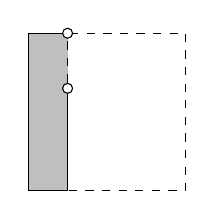
\begin{tikzpicture}
      \draw [dashed] (0,0) rectangle (2,2);
      \fill [lightgray] (0,0) rectangle (0.5,2);
      \node (a) [draw,circle,inner sep=0in,minimum size=0.05in,fill=white] at (0.5,1.3) {};
      \node (b) [draw,circle,inner sep=0in,minimum size=0.05in,fill=white] at (0.5,2) {};
      \draw (b) -- (0,2) -- (0,0) -- (0.5,0) -- (a);
      \draw [dashed] (a) -- (b);
    \end{tikzpicture}

    \(a_{<}\)
  \end{minipage}
  \begin{minipage}{2in}
    \centering
    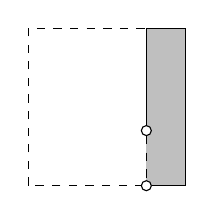
\begin{tikzpicture}
      \draw [dashed] (0,0) rectangle (2,2);
      \fill [lightgray] (1.5,0) rectangle (2,2);
      \node (a) [draw,circle,inner sep=0in,minimum size=0.05in,fill=white] at (1.5,0.7) {};
      \node (b) [draw,circle,inner sep=0in,minimum size=0.05in,fill=white] at (1.5,0) {};
      \draw (a) -- (1.5,2) -- (2,2) -- (2,0) -- (b);
      \draw [dashed] (a) -- (b);
    \end{tikzpicture}

    \(a_{>}\)
  \end{minipage}
  \begin{minipage}{2in}
    \centering
    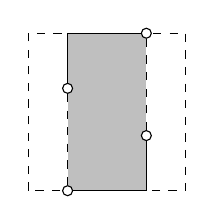
\begin{tikzpicture}
      \draw [dashed] (0,0) rectangle (2,2);
      \fill [lightgray] (0.5,0) rectangle (1.5,2);
      \node (a) [draw,circle,inner sep=0in,minimum size=0.05in,fill=white] at (0.5,1.3) {};
      \node (b) [draw,circle,inner sep=0in,minimum size=0.05in,fill=white] at (1.5,0.7) {};
      \node (c) [draw,circle,inner sep=0in,minimum size=0.05in,fill=white] at (0.5,0) {};
      \node (d) [draw,circle,inner sep=0in,minimum size=0.05in,fill=white] at (1.5,2) {};
      \draw (a) -- (0.5,2) -- (d);
      \draw (b) -- (1.5,0) -- (c);
      \draw [dashed] (a) -- (c);
      \draw [dashed] (b) -- (d);
    \end{tikzpicture}

    \((a,b)\)
  \end{minipage}
\end{example}

\begin{theorem}[3.25]
  Let \((X,\T)\) be a topological space and let \(Y\subset X\).  \(\T_Y\) is a topology on \(Y\).
\end{theorem}

\begin{proof}
  \(\emptyset\cap Y=\emptyset\in\T_Y\) and \(X\cap Y=Y\in\T_Y\).

  Assume \(U,V\in\T_Y\).  Then there exists \(U',V'\in\T\) such that \(U=U'\cap Y\) and \(V=V'\cap Y\).  So:
  \[U\cap V=(U'\cap Y)\cap(V'\cap Y)=(U'\cap V')\cap Y\]
  But \(U'\cap V'\in\T\).  Therefore \(U\cap V\in\T_Y\).

  Now, assume that \(\set{U_{\a}:\a\in\l}\) such that \(U_{\a}\in\T_Y\).  Then for each \(U_{\a}\) there exists a
  \(U_{\a}'\in\T\) such that \(U_{\a}=U_{\a}'\cap Y\).  So:
  \[U=\bigcup_{\a\in\l}U_{\a}=\bigcup_{\a\in\l}(U_{\a}'\cap Y)=\left(\bigcup_{\a\in\l}U_{\a}'\right)\cap Y\]
  But \(\bigcup_{\a\in\l}U_{\a}'\in\T\).  Therefore, \(U\in\T_Y\).

  Therefore \(\T_Y\) is a topology on \(Y\).
\end{proof}

\begin{example}[Exercise 3.26]
  Consider \(Y=[0,1)\) as a subspace of \(\R_{std}\).  In \(Y\), is the set \(\left[\frac{1}{2},1\right)\) open,
  closed, neither, or both?

  There is no open set in \(X\) that will result in a closed endpoint at \(\frac{1}{2}\) so the set is not open.
  However, \([0,1)\cap\left(\frac{1}{2},1\right)=\left(\frac{1}{2},1\right)\in\T_Y\) and \(\frac{1}{2}\) serves as
  a limit point in \(Y\) so \(\left[\frac{1}{2},1\right)\) is closed in \(Y\).  Hence it is not neither and not
  both.
\end{example}

\begin{theorem}[3.28]
  Let \((Y,\T_Y)\) be a subspace of \((X,\T)\).  \(C\subset Y\) is closed in \((Y,\T_Y)\) iff there exists
  \(D\subset X\), closed in \((X,\T)\), such that \(C=D\cap Y\).
\end{theorem}

\begin{proof}
  \begin{description}
  \item[]
  \item[\(\implies\)] Assume \(C\subset Y\) is closed in \((Y,\T_Y)\).

    Since \(C\) in closed in \(Y\), \(Y-C\) is open in \(Y\).  So there exists some \(U\in\T\) such that
    \(Y-C=U\cap Y\).  Let \(D=X-U\), which is closed in \(X\):
    \[D\cap Y=(X-U)\cap Y=(X\cap Y)-(U\cap Y)=Y-(Y-C)=C\]
    Therefore there exists \(D\subset X\), closed in \((X,\T)\), such that \(C=D\cap Y\).

  \item[\(\impliedby\)] Assume there exists \(D\subset X\), closed in \((X,\T)\), such that \(C=D\cap Y\).

    Since \(D\) is closed in \(X\), \(X-D\) is open in \(X\) and \((X-D)\cap Y\) is open in \(Y\):
    \[(X-D)\cap Y=(X\cap Y)-(D\cap Y)=Y-C\]
    Therefore \(C\) is closed in \((Y,\T_Y)\).
  \end{description}
\end{proof}

\end{document}
